%------------------------------------------------
\chapter{Introdução}\label{Introducao}
%---------------------------------------------------------

% Relevância e Aplicação do estudo de dinâmica de estruturas
\section{Relevância e Motivação}
% Vibrações no princípio -
A ideia de transmissão de energia sem fio foi proposta inicialmente por Nikola Tesla, no início do século XX, para alimentar lâmpadas remotamente \cite{TESLA:2000}. Segundo \citeonline{YEAGER:2009}, implementações modernas de sistemas de transmissão de energia remota são implementados de duas formas: indutiva ou radioativa.

Sistemas com acoplamento indutivo utilizam o campo magnético para transmissão de energia. Sistemas desse tipo podem ser observados em aplicações como implantes médicos \cite{SCHUDER:2002}, carregamento de eletrônicos \cite{WELLS:2005}, e a fabricação de salas limpas, utilizadas, por exemplo, no processo de fabricação de \textit{chips} eletrônicos \cite{SALIMIAN:1997}.

Sistemas radioativos, por sua vez, utilizam propagação de ondas de radio-frequência para transmitir energia. Esse método é utilizada para enviar dados em praticamente todos os sistemas de comunicação sem fio \cite{YEAGER:2009}. 

A principal motivação para o uso desse tipo de método está no alcance da transmissão. Segundo \citeonline{YEAGER:2009}, sistemas indutivos possuem melhor rendimento, porém seu alcance está restrito a alguns centímetros, à medida que sistemas radioativos chegam a dezenas de metros. A implementação desse tipo de aplicação é, geralmente, chamada RFID. Algumas aplicações desse tipo de sistema são identificação em sistemas de segurança e pagamento \cite{WEINSTEIN:2005}, monitoramento de animais \cite{YEAGER:2010}, assistência social para idosos \cite{PHILIPOSE:2004}, monitoramento de objetos \cite{RANASHINGHE:2005}, entre outros.

Etiquetas {RFID} passivas somente podem operar com a existência de circuitos que desempenhem o papel de colheita de energia remotamente. A principal motivação deste trabalho é a criação de um circuito que possa permitir o desenvolvimento de etiquetas de forma simples e genérica, contribuindo para a evolução das pesquisas e de trabalhos nessa área.


\section{Descrição do Trabalho}
O trabalho desenvolvido consistiu no projeto teórico e na simulação, a nível de esquemático, de seis módulos que, em conjunto, receberam a denominação de \textit{front-end} analógico. A função desse sistema é coletar energia proveniente de ondas transmitidas por um leitor, em frequência específica, para alimentar um circuito passivo. Os módulos desenvolvidos são, a seguir, listados e, brevemente, descritos.

\begin{itemize}
	\item \textbf{Retificador}: Responsável por ampliar o sinal CA recebido na entrada e retificá-lo, de modo a fornecer a tensão apropriada aos demais módulos, que operam em CC. A tensão aqui fornecida não é regulada e seu valor não é preciso;
	\item \textbf{Referencial de Corrente}: Estabelece níveis de corrente de 50 nA utilizados na polarização de transistores que operam como fonte de corrente;
	\item \textbf{Referencial de Tensão de 0,7 V}: Responsável por fornecer um nível de tensão fixo de 0,7 V para o regulador de tensão;
	\item \textbf{Referencial de Tensão de 1,2 V}: Responsável por fornecer um nível de tensão fixo de 1,2 V para o regulador de tensão;
	\item \textbf{Regulador de Tensão}: Módulo que servirá como fonte de tensão no valor do referencial utilizado;
\end{itemize}


\section{Revisão da Literatura}
Esta seção apresenta uma breve revisão de pontos importantes para a compreensão do trabalho realizado. São tratados, de forma superficial, a tecnologia {RFID}, a teoria sobre colheita de energia sem fio e a tecnologia {CMOS}. No fim, são apresentados os módulos fundamentais para um \textit{front-end} analógico.

\subsection{Tecnologia RFID}
Sistemas RFID consistem, tipicamente, de um leitor que emite um sinal de radiofrequência e de um transceptor, comumente chamado etiqueta. Estas, por sua vez, são dispositivos tipicamente pequenos e de baixo custo, que usam o sinal para alimentação e comunicação. As etiquetas são fixadas aos pontos de interesse e as informações necessárias são obtidas e retransmitidas ao leitor quando assim requisitado.

As etiquetas possuem uma antena para capturar energia de radiofrequência, um retificador para extração de potência {CC} e circuitos de processamento e comunicação que são alimentados dessa potência {CC} \cite{MANDAL:2007}. Essas etiquetas são classificadas, principalmente, de acordo com a alimentação. Elas podem ser ativas, quando alimentadas por uma fonte dedicada, semi-passivas, se assistidas por uma fonte não totalmente independente, ou passivas, quando não contam com fonte dedicada de alimentação. Este trabalho foca em etiquetas passivas e as análises e comentários doravante realizados referem-se a esse tipo de dispositivo.

Atualmente, etiquetas e leitores radioativos de longo alcance disponíveis no mercado utilizam, principalmente, o padrão \textit{Class 1 Generation 2 UHF Air Interface Protocol Standard}, da \textit{Electronic Product Code} (EPC) \cite{EPCGLOBAL:2009}. Anteriormente conhecido como ISO/IEC 18000-6 Tipo-C e, informalmente, chamado de \textit{Gen2}, esta especificação define as camadas de rede e de protocolo para comunicação {RFID} \cite{YEAGER:2009}. Outras especificações são fornecidas pela {EPCGlobal}, como a organização dos dados das etiquetas e a comunicação entre elas e os leitores. Essas especificações têm o objetivo de prover interoperabilidade entre fabricantes e uniformidade aos usuários.

Etiquetas passivas costumam requerer pelo menos $-20~dBm$ de potência de entrada para gerar energia suficiente para operar. Segundo \citeonline{YEAGER:2009} os leitores tipicamente transmitem sinais de radiofrequência no limite da regulação de $1~W$ ($30~dBm$). Isso permite até $50~dBm$ de perda no caminho. Assumindo a mesma perda na retransmissão do sinal, o leitor recebe o sinal retransmitido com $-70~dBm$. Tipicamente se constroem leitores com sensibilidade de $-80~dBm$, a fim de garantir performance. Como esses dispositivos são fixos e possuem alimentação garantida, é possível que isso aconteça, ao contrário das etiquetas passivas que dependem das ondas incidentes para alimentação.

A baixa potência retransmitida pelas etiquetas unida à baixa sensibilidade de seus receptores torna impraticável a comunicação entre etiquetas. Por outro lado, como leitores possuem emissores de alta potência e sensibilidade elevada, a comunicação entre eles é viável. Ao mesmo tempo, caso dois leitores diferentes estejam utilizando o mesmo canal de comunicação, um pode bloquear o outro de interpretar os sinais de resposta de etiquetas. É importante, portanto, que leitores localizados próximos utilizem canais diferentes na comunicação. \citeonline{EPCGLOBAL:2009} apresenta a largura de banda dos canais no padrão.

As etiquetas são dispositivos simples. A comunicação entre elas e leitores ocorre através de retroespalhamento do sinal incidente, proveniente do leitor. Portanto, a resposta das etiquetas é dada no mesmo canal do sinal incidente. Consequentemente, os leitores somente se comunicam em seu próprio canal. Outra característica devida à simplicidade no desenvolvimento das etiquetas é que elas são incapazes de distinguir leitores. Como os sinais de radiofrequência recebidos são misturados na entrada e passam por um processo de retificação, não há como a etiqueta diferenciar os sinais pela frequência de canal utilizada. O processo de diferenciação pode ser implementado com técnicas específicas para este fim, como a utilização de sessões diferentes ou a inclusão desta informação na mensagem transmitida.

A comunicação nessa tecnologia é sempre iniciada pelo leitor. Em alguns casos, a etiqueta sequer responde, somente quando assim requisitado. Para casos em que há constante troca de informações entre leitor e etiqueta, como em sensoriamento, essa técnica é ineficiente, devido à grande necessidade de requisições por parte do leitor.

A comunicação entre leitor e etiqueta é realizada através de códigos únicos de identificação (IDs). A cada etiqueta é atribuído um ID e esse é informado ao leitor na primeira comunicação entre eles. Caso o leitor já conheça o ID de alguma etiqueta, ele pode se comunicar diretamente com ela. O descobrimento de novas etiquetas é um processo estocástico \cite{YEAGER:2009}.


\subsection{Colheita de Energia}
Colheita de energia é o processo pelo qual a energia elétrica é extraída de fontes externas (solar, eólica, térmica, cinética etc), capturada e utilizada para alimentar dispositivos eletrônicos autônomos de baixa potência \cite{BEEBY:2010} \cite{PRIYA:2009}.

Etiquetas RFID passivas operando na faixa UHF recebem energia através do campo eletromagnético irradiado. A distância limite entre os campos próximo e distante para essas etiquetas, operando entre 868 MHz e 915 MHz, é de pouco mais de 5 centímetros. Devido à pequena diferença de alcance observada, etiquetas RFID UHF operam, quase sempre, em campo distante. Esse modo de operação significa dizer que a frequência da portadora é a máxima possível. A potência total recebida na antena da etiqueta pode ser calculada a partir da Equação da Transmissão de Friis, apresentada em (\ref{eq:friis}).

\begin{equation}
	\label{eq:friis}
	P_{etiqueta}~=~P_{leitor} \cdot G_{leitor} \cdot G_{etiqueta} \cdot \Big ( \dfrac{\lambda}{4 \pi d} \Big )^2
\end{equation}

Nessa equação, $d$ é a distância entre as antenas do leitor e da etiqueta, $\lambda$ o comprimento de onda da portadora, $P_{leitor}$ a potência transmitida pelo leitor e $G_{leitor}$ e $G_{etiqueta}$ os ganhos das antenas do leitor e da etiqueta, respectivamente.

\begin{figure}[!htb]
	\caption{\label{fig:intro}Máxima potência disponível para etiqueta RFID operando em 915 MHz}
	\begin{center}
		\includegraphics[width=0.9\linewidth]{intro.png}
	\end{center}
	\legend{Fonte: autor}
\end{figure}

Considerando o produto $P_{leitor} \cdot G_{leitor}$ igual a $33~dBm$, que é a máxima potência radiada equivalente (PERP) permitida pelas regulamentações americana e europeia, $G_{etiqueta}$ igual a $-3~dBi$, $0~dBi$ e $+3~dBi$ e $f~=~915~MHz$ ($\lambda~=~0,3276~m$), pode-se estimar a potência disponível para uma etiqueta UHF distante entre 0 e 30 m da antena do leitor conforme representado na Figura \ref{fig:intro}.

A análise do gráfico permite estimar a faixa de energia disponível para o funcionamento de uma etiqueta RFID UHF operando a uma dada distância da antena do leitor. A 18 metros, por exemplo, a potência recebida na etiqueta será, no melhor dos casos ($G_{etiqueta}~=~+3~dBi$), igual a $-20,783~dBm$, ou seja, cerca de $8,35~\mu W$.

O projeto de um sistema de colheita de energia capaz de operar satisfatoriamente com potências dessa magnitude requer tecnologia, técnicas e abordagens apropriadas para que o próprio circuito de colheita não consuma por si mesmo a energia captada. Várias soluções para esse problema têm sido propostas na literatura científica nos últimos anos. A solução que se pretende implementar neste trabalho é baseada na proposta por \citeonline{YEAGER:2009}.


\subsection{Tecnologia CMOS}
Nas últimas cinco décadas, circuitos digitais evoluíram drasticamente, passando desde algumas portas por \textit{chip} nos anos 60 a centenas de milhões de transistores por \textit{chip} hoje \cite{HAZAVI:2008}. Existem, atualmente, diversas soluções para a produção de circuitos integrados, como TTL, ECL, CMOS e BiCMOS. Dentre elas, o CMOS - \textit{Complementary MOS} - é, de longe, a tecnologia mais popular para a implementação de sistemas digitais \cite{SEDRA:2007}. Alguns dos motivos que levaram à larga utilização dessa tecnologia são:

\begin{itemize}
	\item Menor dissipação de potência por aquecimento (efeito Joule), possibilitando a redução das áreas dos circuitos integrados;
	\item Alta impedância de entrada, permitindo o armazenamento temporário de informações para aplicações em circuitos lógicos e memórias;
	\item A dimensão mínima dos componentes MOS tem diminuído muito ao longo dos anos. Hoje já existem processadores no mercado que utilizam tecnologia de produção de 14 nm \cite{INTEL:2015}.
\end{itemize}

A tecnologia CMOS, como leva a induzir por seu nome, é caracterizada pela utilização de NMOS e PMOS simultaneamente no circuito. No que diz respeito a esse tipo de dispositivo, um importante conceito é o de tensão de limiar, comumente representada por $V_T$. Segundo \citeonline{ALLEN:2002}, quando a diferença de tensão entre o porta e o fonte do transistor alcança esse valor, o substrato abaixo do porta é invertido, isto é, ele muda de tipo-p para tipo-n. Consequentemente, um canal tipo-n existe entre o fonte o dreno, permitindo a passagem dos condutores de carga. Segundo \citeonline{MARTIN:1997}, à medida que $v_{GS}$ aumenta, a densidade desses portadores aumenta, proporcionalmente a $v_{eff}~=~v_{GS}~-~V_T$, comumente chamada de tensão porta-fonte eficaz. Essa condição é conhecida como inversão forte, ou região ativa, e é a região de operação preferível para a maior parte de aplicações de transistores tipo MOS.

Os processos de fabricação de dispositivos {CMOS} são classificados, dentre outros critérios, de acordo com o limite inferior de comprimento de canal. À medida que os valores de comprimento ($L$) e largura ($W$) de canal se aproximam dos limites da tecnologia, a previsão do comportamento do dispositivo passa a ser menos trivial. Quando os valores de $L$ e $W$ são grandes (tipicamente a partir de cerca de 10x maiores que os valores mínimos da tecnologia), pode-se utilizar, segundo \citeonline{ALLEN:2002}, (\ref{eq:cmos_active}) para prever o comportamento do dispositivo, quando operando em inversão forte.

\begin{equation}
	\label{eq:cmos_active}
	i_D~=~\dfrac{\mu_oC_{ox}W}{L} \Big [ (v_{GS}~-~V_T)~-~\Big ( \dfrac{v_{DS}}{2} \Big ) \Big ] v_{DS}
\end{equation}

Nessa equação, as os símbolos utilizados dizem respeito a:
\begin{itemize}
	\item $i_D$ - corrente que atravessa o transistor
	\item $\mu_o$ - mobilidade de superfície de canal, para o dispositivo de canal N ou canal P ($\dfrac{cm^2}{V \cdot s}$)
	\item $C_{ox}$ - capacitância por unidade de área do óxido do porta ($\dfrac{F}{cm^2}$)
	\item $W$ - largura de canal efetiva
	\item $L$ - comprimento de canal efetivo
	\item $v_{GS}$ - diferença de potencial entre o porta e o fonte do dispositivo
	\item $V_T$ - tensão de limiar do dispositivo
	\item $v_{DS}$ - diferença de potencial entre o dreno e o fonte do dispositivo
\end{itemize}

Essa aproximação para a modelagem de dispositivos {CMOS} é aceitável para as primeiras etapas de planejamento. Contudo, ferramentas computacionais utilizam modelos com maior nível de precisão, a fim de garantir resultados com maior exatidão e confiabilidade. Essas ferramentas devem ser utilizadas para o projeto dos transistores e para sua simulação, à medida que o projeto avança.

Com a redução do comprimento de canal do transistor, aproximando-se do limite da tecnologia, um fenômeno passa a ser mais perceptível, conhecido como efeito de modulação de comprimento do canal. Como sugere o nome, o que se observa é que o comprimento efetivo de canal do dispositivo é alterado. Na prática, o transistor acaba tendo seu canal comprimido devido a uma maior concentração de portadores na região próxima do fonte do dispositivo. Segundo \citeonline{MARTIN:1997}, uma equação que leva esse efeito em conta é apresentada em (\ref{eq:cmos_active_channel}). Nela, $\lambda$ é denominada constante de impedância de saída e tem unidade de $V^{-1}$ e representa o efeito de modulação de comprimento do canal.

\begin{equation}
	\label{eq:cmos_active_channel}
	i_D~=~\dfrac{\mu_oC_{ox}W}{2L} (v_{GS}~-~V_T)^2 [ 1 + \lambda( v_{DS} - v_{eff} ) ]
\end{equation}

A operação em região ativa, ou inversão forte, contudo, não é prática para situações onde energia é uma variável crítica. Para esses casos, é preferível que o dispositivo opere da forma mais econômica possível, de modo a evitar gastos desnecessários. Em situações assim, o comum é que se projete o transistor para que ele opere em região de sub-limiar, ou inversão fraca.

\begin{citacao}
	Se $v_{eff}~<~-100~mV$, o transistor está em inversão fraca e diz-se que ele está operando na região de sub-limiar. Nessa região, o transistor é mais precisamente modelado por uma relação exponencial entre sua tensão de controle e corrente, de forma similar a um transistor bipolar. Quando nessa região, a corrente de dreno é dada, aproximadamente, por (\ref{eq:cmos_subthreshold}) \cite{MARTIN:1997}.
\end{citacao}

\begin{equation}
	\label{eq:cmos_subthreshold}
	i_D~=~i_{D0} \Big ( \dfrac{W}{L} \Big ) e^{(\dfrac{q v_{GS}}{nKT})}
\end{equation}

Nessa equação, $n~=~\dfrac{C_{ox}+C_{depl}}{C_{ox}}$, onde $C_{depl}$ remete à capacitância por unidade de área da região de depleção do canal do transistor. Para a tecnologia utilizada, testes realizados mostraram que os valores de $n$ para os transistores básicos de canal N variam entre $1,09$ e $1,2$ e para os de canal P variam entre $1,25$ e $1,45$. Os testes foram feitos com transistores de largura de $10~\mu m$ e comprimento variando entre $10~\mu m$ e $120~nm$.

\subsection{Módulos Projetados}
A seguir são apresentados os módulos primordiais para o projeto de um \textit{front-end} analógico. Eles são responsáveis por coletar energia elétrica das ondas eletromagnéticas captadas pela antena do dispositivo. Essa energia é, então, fornecida aos dispositivos da etiqueta para a realização de suas funções.

\subsubsection{Retificador}
\begin{citacao}
	O primeiro passo para se fazer funcionar qualquer sistema remotamente alimentado é energizá-lo. O retificador, nesses sistemas, deve extrair potência {CC} suficiente de radiação eletromagnética incidente para que o dispositivo funcione. A retificação é difícil quando os níveis de potência incidente são baixos. Todos os retificadores possuem uma zona morta não-responsiva para baixa tensão de entrada e técnicas de redução dessa zona morta são difíceis de se implementar, uma vez que não há fonte de alimentação disponível. Fundamentalmente, isso acontece porque a retificação é uma operação não linear e todos os sistemas físicos e dispositivos parecem lineares para pequenos sinais.
\end{citacao}

O retificador consiste num módulo responsável por prover toda a potência necessária para o funcionamento da etiqueta. Alta eficiência, baixo custo no casamento de impedância entre antena e retificador, baixa resistência de saída e alta capacitância de entrada são importantes objetivos a serem alcançadas no projeto de um circuito retificador \cite{BARNETT:2006}.

A potência de entrada disponível para etiquetas está, costumeiramente, entre $-10~dBm$ e $-20~dBm$. Retificadores operando nestes limites de potência estão entre a região linear \cite{DICKSON:1976}, onde a tensão de saída da antena é proporcional à tensão de entrada, e a região quadrática \cite{AGILENT:1999}, onde a tensão de saída da antena é proporcional à potência recebida. Uma análise da tensão de saída de um único diodo retificador é apresentada em \citeonline{HARRISON:1992}.

Segundo \citeonline{BARNETT:2006}, há três métodos de casamento de impedância que podem ser utilizados para alcançar alta eficiência na retificação de um sinal de radiofrequência: casamento com transformador, casamento com indutor e ajuste de indutor \textit{shunt}. O primeiro é difícil devido aos custos de implementação, que são muito elevados para aplicação em etiquetas RFID. O casamento com indutor utiliza um componente série e, possivelmente, elementos adicionais para ressonar a impedância de entrada do dispositivo. O método de casamento com indutância \textit{shunt} necessita de apenas um componente indutivo. Contudo, esse método requer alta precisão na estimação da impedância de entrada do dispositivo.

Para aplicações {RFID}, um retificador multinível geralmente é necessário para obtenção de um nível {CC} aceitável. O alto número de componentes nessa configuração faz variar consideravelmente as características de resistência e capacitância de entrada do elemento \cite{BARNETT:2006}.


\subsubsection{Referenciais de Corrente e Tensão}
\begin{citacao}
	Uma fonte de corrente é um componente de dois terminais cuja corrente, em qualquer instante, é independente da tensão entre seus terminais. O fluxo de corrente nesse dispositivo segue do terminal positivo ao negativo. [...] Ao porta é atribuído o nível de tensão necessário para criar o valor desejado de corrente. [...] Nota-se que na região de não-saturação, um dispositivo MOS não é uma boa fonte de corrente. A tensão entre os terminais de uma fonte de corrente deve ser maior que sua tensão mínima de saturação. \cite{ALLEN:2002}.
\end{citacao}

Circuitos {CMOS} que fornecem correntes em níveis específicos são chamados fontes e drenos de corrente. A \autoref{fig:current_source_sink} apresenta as configurações básicas desses elementos. Nesses elementos, a tensão $V_{ref}$ polariza os transistores de modo que a corrente desejada $I_{saída}$ circule por seus terminais.

\begin{figure}[!htb]
	\caption[Esquemas de fonte e dreno de corrente]{\label{fig:current_source_sink}Esquemas de fonte e dreno de corrente}
	\begin{center}
		\subfloat[Fonte de corrente]{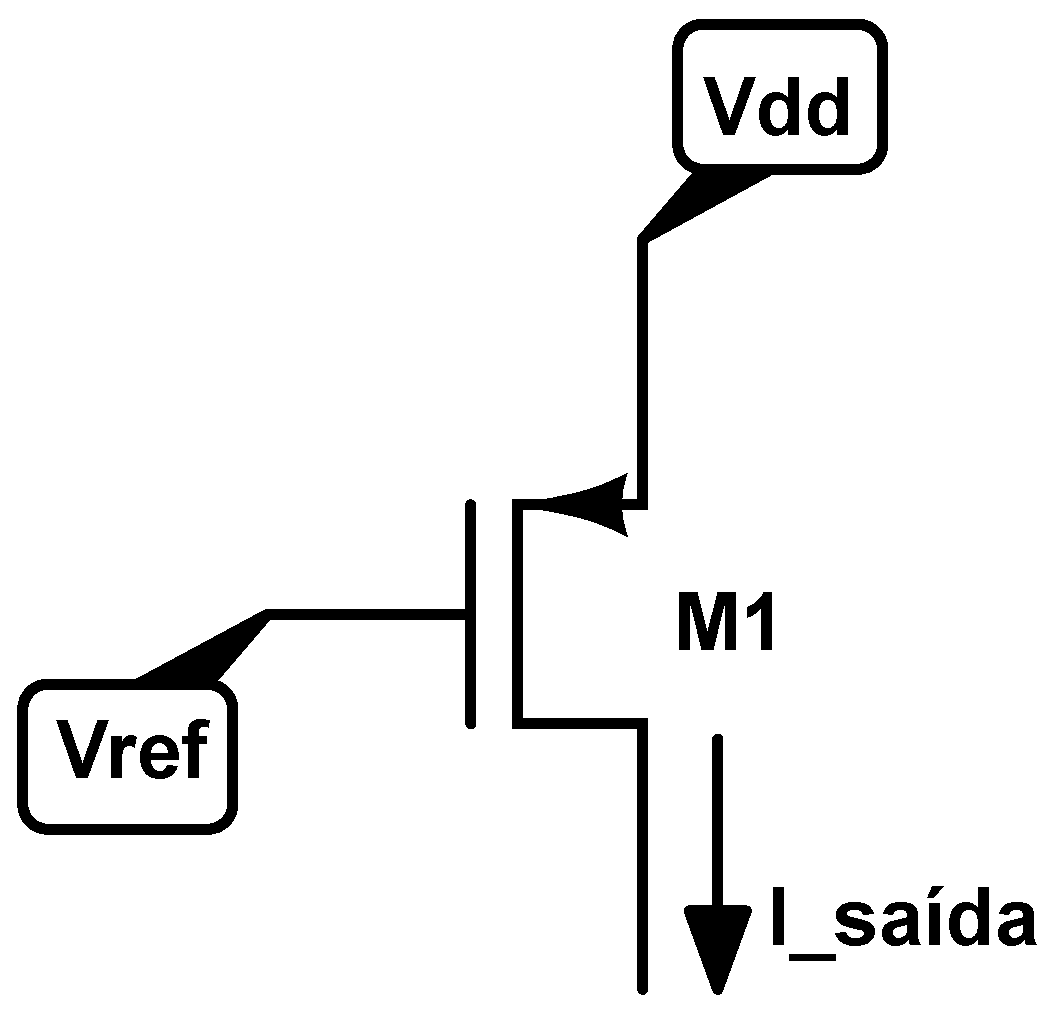
\includegraphics[width=0.3\linewidth]{current-source.eps}}
		\hspace*{0.1\linewidth}
		\subfloat[Dreno de corrente]{\includegraphics[width=0.3\linewidth]{current-sink.eps}}
	\end{center}
	\legend{Fonte: adaptado de \citeonline{ALLEN:2002}}
\end{figure}

Uma técnica utilizada para a redução da tensão de saturação do sistema e acréscimo na impedância da fonte de corrente é a utilização de configuração em cascata, como as apresentadas na \autoref{fig:current_source_sink_cascode}. Nesse esquema são necessárias duas referências $V_{ref1}$ e $V_{ref2}$ para a polarização dos transistores. A maior robustez dessa configuração é devida à menor oscilação no nível de $I_{saída}$ pelo acréscimo do segundo estágio de polarização.

\begin{figure}[!htb]
	\caption{\label{fig:current_source_sink_cascode}Esquemas de fonte e dreno de corrente com configuração em cascata}
	\begin{center}
		\subfloat[Fonte de corrente em cascata]{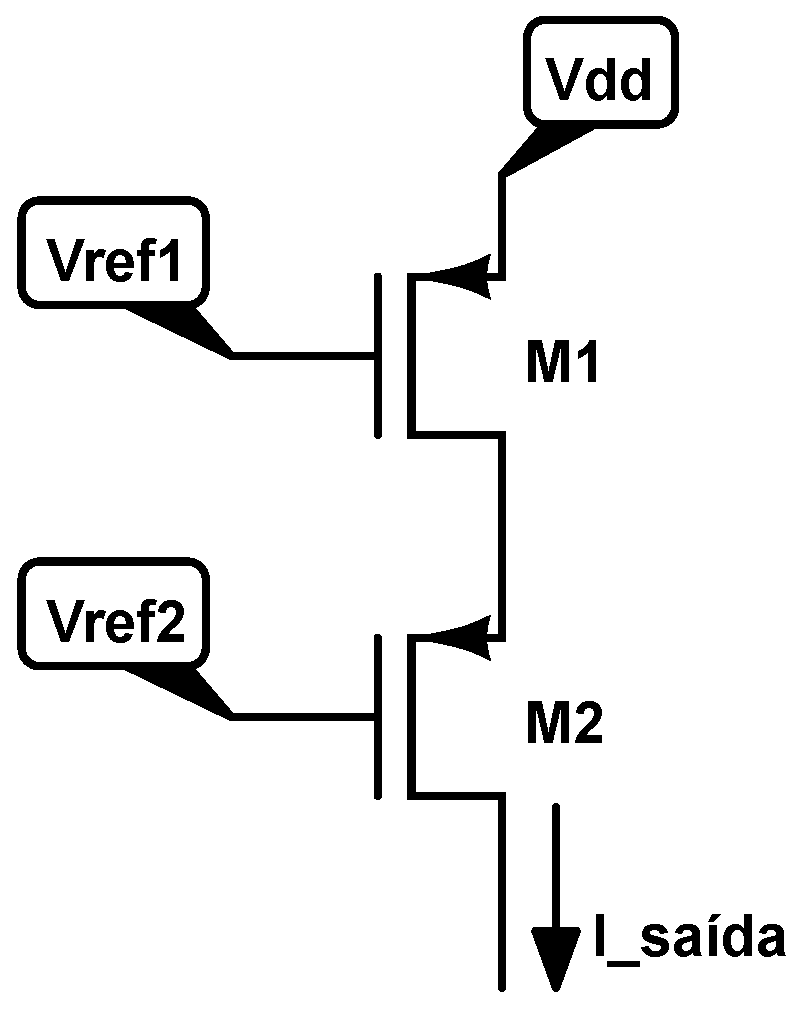
\includegraphics[width=0.3\linewidth]{current-source-cascode.eps}}
		\hspace*{0.1\linewidth}
		\subfloat[Dreno de corrente em cascata]{\includegraphics[width=0.3\linewidth]{current-sink-cascode.eps}}
	\end{center}
	\legend{Fonte: adaptado de \citeonline{ALLEN:2002}}
\end{figure}

Espelhos de corrente são simplesmente extensões de fontes de corrente \cite{ALLEN:2002}. O princípio base desse tipo de circuito é o de que se os portas dos transistores estiverem sob o mesmo potencial, a corrente que fluirá sobre os dispositivos é a mesma. Um exemplo de espelho de corrente com configuração em cascata utilizando transistores de canal P é apresentada na \autoref{fig:current_mirror_cascode}. Para essa configuração, os referenciais de tensão de {M1} e {M2} são fornecidos por {M3} e {M4}, respectivamente, que são polarizados por uma corrente de referência $I_{ref}$. Idealmente, para esse circuito, $I_{saída}~=~I_{ref}$.

\begin{figure}[!htb]
	\caption{\label{fig:current_mirror_cascode}Espelho de corrente com configuração em cascata}
	\begin{center}
		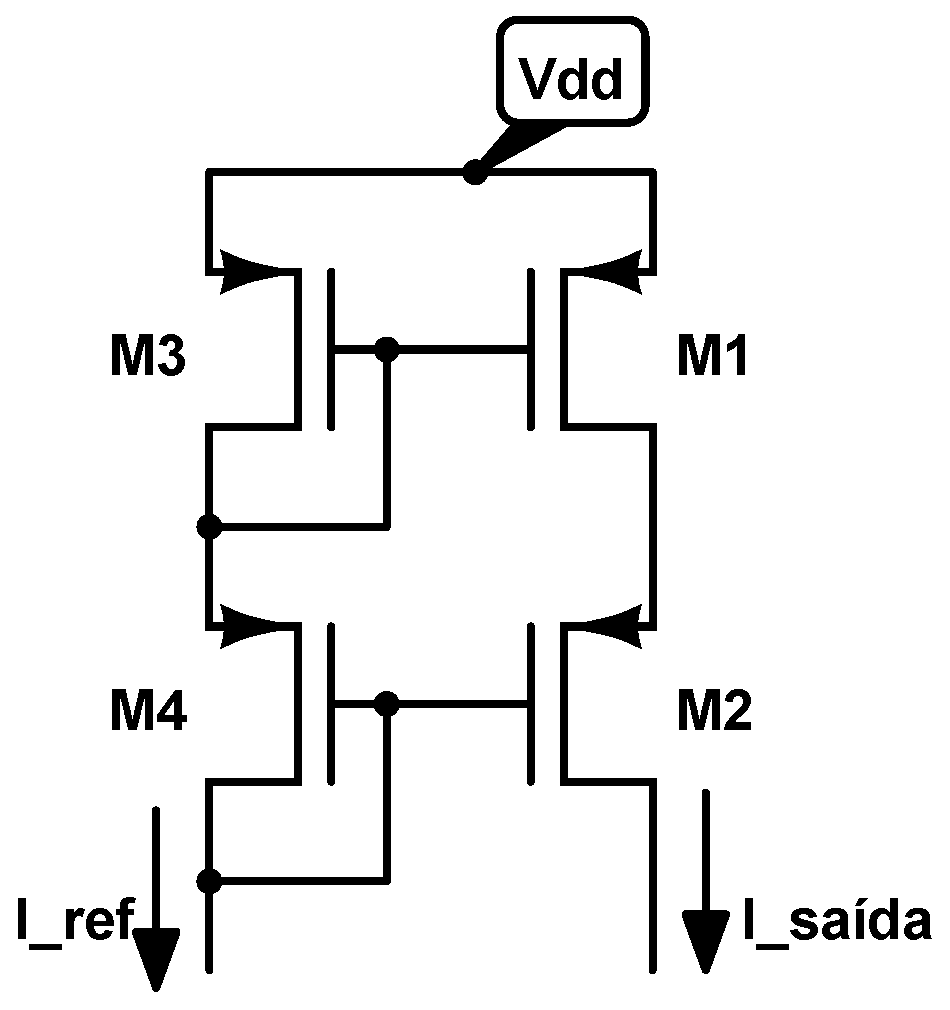
\includegraphics[width=0.5\linewidth]{current-mirror-cascode.eps}
	\end{center}
	\legend{Fonte: adaptado de \citeonline{ALLEN:2002}}
\end{figure}

Um referencial de corrente é um circuito que estabelece níveis específicos de tensão a fim de polarizar transistores que conduzirão correntes em valores desejados. Uma vez alcançado este ponto, fontes podem ser geradas com a utilização de espelhos de corrente. Referenciais de corrente são, idealmente, independentes de temperatura e tensão de alimentação.

De forma análoga a um referencial de corrente, um referencial de tensão é um circuito responsável por estabelecer níveis específicos de tensão. A independência de fonte de alimentação e temperatura é uma característica desejável, também, nesses circuitos. O projeto desse tipo de circuito segue a mesma filosofia de um referencial de corrente, excetuando-se a polarização dos transistores que agiriam como fonte de corrente.

\begin{citacao}
	O princípio de independência da temperatura é bastante simples. Ele tem início com a identificação de uma tensão que aumente com a temperatura e outra que diminua. [...] A tensão que aumenta é chamada \textit{Proportional to Absolute Temperature} ou PTAT e a que diminui é chamada \textit{Complementary to Absolute Temperature} ou CTAT. Em seguida, a tensão com a menor inclinação de curva é multiplicada por uma constante $K$ de modo que a inclinação resultante seja igual. Finalmente, se ambas forem somadas, a tensão resultante deverá ser independente da temperatura. \cite{ALLEN:2002}.
\end{citacao}


\subsubsection{Regulador de Tensão}
Reguladores de tensão são dispositivos responsáveis por fornecer níveis específicos de tensão para alimentação de outros equipamentos. Pode-se entendê-los como fontes de tensão no circuito.

Os circuitos referenciais de tensão são, de forma geral, incapazes de serem utilizados como fonte de alimentação. Seus projetos são realizados com alta impedância de saída em vista, impossibilitando sua aplicação nesse campo. Para esse objetivo, utilizam-se circuitos reguladores de tensão.

Circuitos reguladores necessitam de referenciais para gerar os valores desejados de tensão. Isso pode ser atingido com a aplicação de amplificadores operacionais. A utilização de um amplificador simples de um estágio, como o apresentado na \autoref{fig:ampop_one_stage}, operando em região de sub-limiar, deixa de ser prática a partir de um determinado nível de tensão de alimentação. Nesse tipo de circuito, o ganho é expresso como mostra (\ref{eq:ganho_a}), onde $\lambda_{Dn}$ e $\lambda_{Dp}$ representam constantes características dos transistores de canal N ({M1} e {M2}) e de canal P ({M3} e {M4}) da configuração do amplificador, respectivamente.

\begin{figure}[!htb]
	\caption{\label{fig:ampop_one_stage}Amplificador operacional de um estágio}
	\begin{center}
		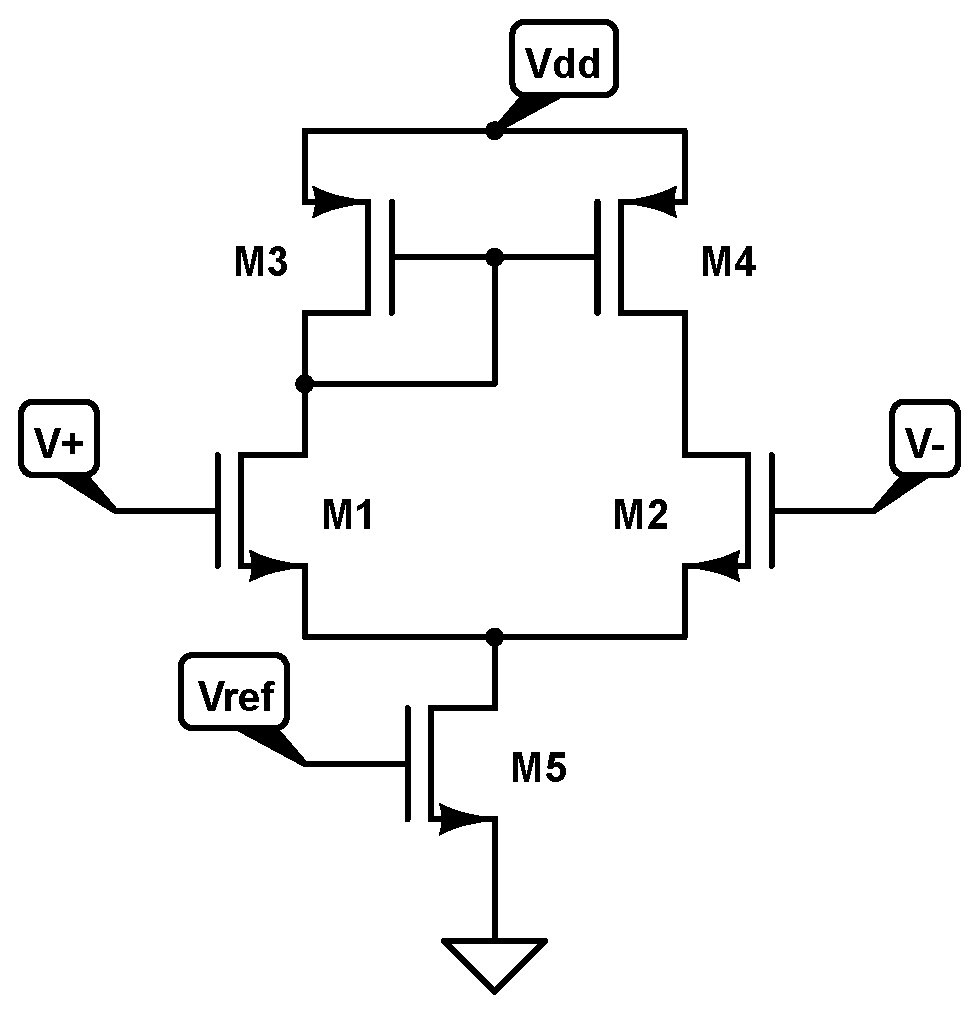
\includegraphics[width=0.45\linewidth]{ampop-single-stage.eps}
	\end{center}
	\legend{Fonte: autor}
\end{figure}

\begin{figure}[!htb]
	\caption{\label{fig:ampop_one_stage_cascode}Amplificador operacional de um estágio em cascata}
	\begin{center}
		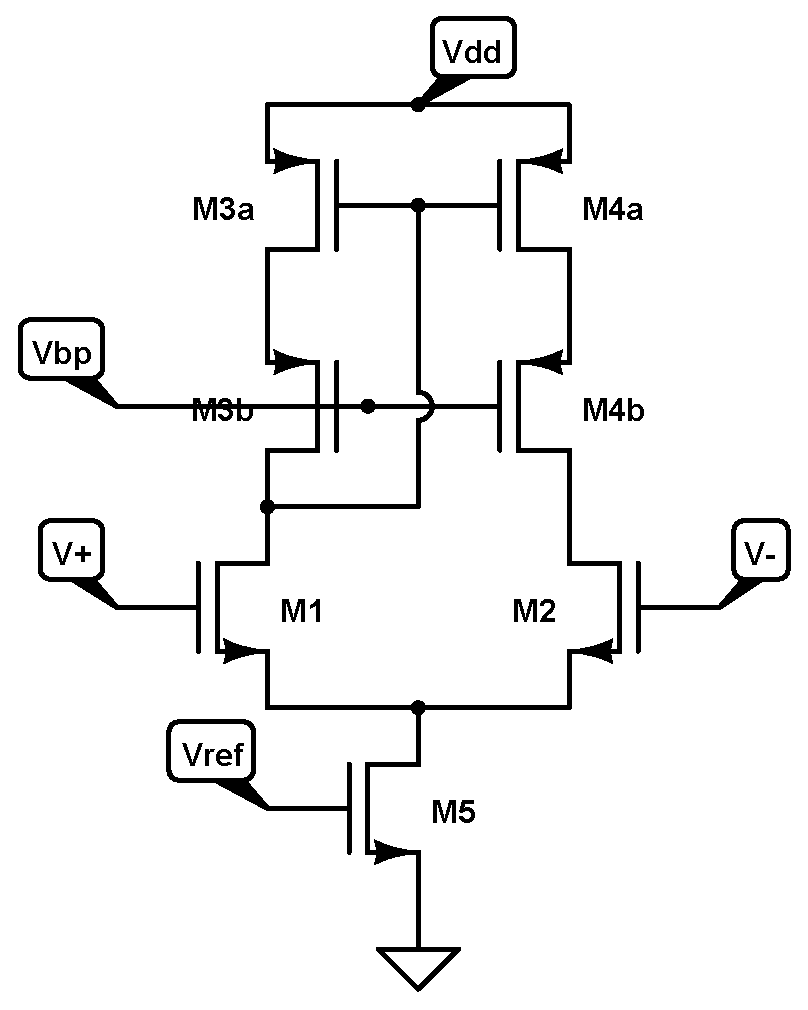
\includegraphics[width=0.45\linewidth]{ampop-single-stage-cascode.eps}
	\end{center}
	\legend{Fonte: autor}
\end{figure}

\begin{equation}
	\label{eq:ganho_a}
	A_V~=~\dfrac{1}{\lambda_{Dn}~+~\lambda_{Dp}}
\end{equation}

Para a tecnologia utilizada neste trabalho, o valor de $\lambda_{Dn}$ decresce com o aumento da tensão entre os terminais do transistor até certo ponto. A partir desse ponto seu valor aumenta, reduzindo o ganho do sistema.

A fim de contornar esse problema, uma configuração em cascata, como a utilizada neste trabalho, pode ser implementada. Esse tipo de configuração é apresentado na \autoref{fig:ampop_one_stage_cascode}. Nela, devido à cascata, a queda de tensão entre a alimentação $V_{dd}$ e o NMOS {M1} é aumentada. Dessa forma, reduz-se a tensão que deve ser dividida entre os transistores de canal N do amplificador, reduzindo, portanto, o valor de $\lambda_{Dn}$.


\section{Metodologia}
O estudo realizado consistiu no projeto CMOS dos módulos necessários, utilizando como ponto de partida as análises feitas por \citeonline{YEAGER:2009}. A arquitetura escolhida para o desenvolvimento do núcleo analógico foi a mesma. Os módulos foram desenvolvidos seguindo os mesmos esquemáticos.

As dimensões dos transistores utilizados foram definidas a partir de análises teóricas, tendo como prioridade a minimização do consumo de energia, visto sua baixa disponibilidade para as etiquetas.

Uma vez projetados os módulos, foram realizadas simulações em ambiente \textit{Cadence Virtuoso} a fim de validar os projetos propostos. Correções necessárias foram aplicadas durante as simulações.

Após as validações dos módulos de forma individual, foram realizados testes com todos em conjunto, a fim de validar o projeto como um todo.


\section{Objetivos}
A seguir são apresentados os objetivos desejados com o estudo realizado. É apresentado, inicialmente, o objetivo geral deste trabalho e, em seguida, listam-se objetivos específicos que se desejam alcançar.

\subsection{Objetivo Geral}
Desenvolver um \textit{front-end} analógico para a colheita de energia eletromagnética, na faixa UHF, destinado a alimentar uma etiqueta RFID passiva.

\subsection{Objetivos Específicos}
Os objetivos específicos que se deseja alcançar com o trabalho são os seguintes:

\begin{itemize}
	\item Dominar as ferramentas e recursos necessários ao projeto de sistemas de radiofrequência integrados em tecnologia IBM CMOS 8RF 130 nm para a faixa UHF (820 a 960 MHz);
	\item Desenvolver o sistema de forma genérica, para que ele possa, facilmente, ser integrado em futuras aplicações de áreas diversas.
\end{itemize}


\section{Estrutura do Trabalho}
Este trabalho é estruturado em quatro capítulos, conforme as descrições que seguem:

\begin{itemize}
	\item \textbf{Capítulo 01}: Introdução acerca do tema tratado, motivação do estudo e contextualização do tema na sociedade atual;
	\item \textbf{Capítulo 02}: Neste capítulo são realizadas análises específicas sobre cada um dos módulos implementados e são apresentadas as informações presentes na literatura sobre eles;
	\item \textbf{Capítulo 03}: Apresenta os módulos projetados e os resultados observados em suas simulações, bem como observações pertinentes acerca desses resultados;
	\item \textbf{Capítulo 04}: São apresentadas, sucintamente, as principais conclusões observadas no trabalho, além de sugestões para futuros trabalhos nessa linha.
\end{itemize}